\documentclass[12pt]{amsart}
\usepackage[letterpaper, portrait, left = 1in, right = 1in, top = 1.2in, bottom=1.5in]{geometry} 
%\usepackage{setspace} \doublespacing
%\usepackage[letterpaper, portrait, margin=1.3in]{geometry}
\usepackage[table,xcdraw]{xcolor}
\usepackage{amssymb}
\usepackage{amsfonts}
\usepackage{longtable}
\usepackage{amsmath,amsthm}
\usepackage{enumitem}
\usepackage[utf8]{inputenc}
\usepackage{mathtools}
\usepackage{graphicx}
\usepackage{parskip}
\usepackage{multicol}
\usepackage{listings}
\usepackage[skip=0.25pt]{caption}
\usepackage[mathscr]{euscript}
\usepackage{quiver}
\setlength{\parindent}{0pt}
\usepackage{thm-restate}
\definecolor{vividburgundy}{rgb}{0.62, 0.11, 0.21}
\usepackage[driverfallback=hypertex,pagebackref=false,colorlinks,citecolor=vividburgundy]{hyperref}
\usepackage[capitalize]{cleveref}
%\usepackage[cmintegrals,cmbraces]{newtxmath}
%\usepackage{ebgaramond-maths}

%\usepackage{fourier}
%----------FONT OPTIONS----------
% sans-serif
%\usepackage[sfdefault]{FiraSans}
 %\usepackage[sfdefault]{roboto}
% \usepackage[sfdefault]{noto-sans}
%\usepackage[default]{sourcesanspro}

% serif
%\usepackage{CormorantGaramond}

%\usepackage{charter}
\usepackage[T1]{fontenc}
\usepackage{cleveref}
\definecolor{dg}{RGB}{10, 100, 10}
\setlength{\parindent}{0in}
\renewcommand{\qed}{$\hfill\blacksquare$}
% \newtheoremstyle{style}{2pt}{1pt}{\normalfont}{}{\bfseries}{\\}{0cm}{}
% \theoremstyle{style}
\newtheorem{lemma}{Lemma}[section]
% \newtheorem{lemma}{Lemma}
\newtheorem{thm}[lemma]{Theorem}
\newtheorem{prop}[lemma]{Proposition}
\newtheorem{cor}[lemma]{Corollary}
\newtheorem{conj}[lemma]{Conjecture}
\newtheorem{cl}[lemma]{Claim}
\newtheorem{rmk}{Remark}
\newtheorem{defn}[lemma]{Definition}
\newtheorem{qs}{Question}
\newtheoremstyle{styleS}{}{}{\color{dg}}{}{\color{dg}\bfseries}{. }{0cm}{}
\theoremstyle{styleS}
\newtheorem*{sol}{Solution}
\newtheoremstyle{style1}{}{}{\normalfont}{}{\bfseries}{. }{0cm}{}
\theoremstyle{style1}
\newtheorem{prob}{Problem}[section]
\newtheorem*{prb}{Problem}
\newtheoremstyle{style2}{1pt}{4pt}{\normalfont}{}{\itshape}{. }{0cm}{}
\theoremstyle{style2}
\newtheorem{ex}[lemma]{Example}
\newtheorem*{pf}{Proof}

\newcommand{\norm}[2]{
\left\lVert #1 \right\rVert_{#2}
}
\usepackage{mathrsfs}
%\usepackage[table,xcdraw]{xcolor}
\usepackage{booktabs}
\usepackage{tikz}
\usetikzlibrary{matrix}
\renewcommand{\l}{\ell}


\newcommand{\fA}{{\mathfrak{A}}}   \newcommand{\fB}{{\mathfrak{B}}}
\newcommand{\fC}{{\mathfrak{C}}}   \newcommand{\fD}{{\mathfrak{D}}}
\newcommand{\fE}{{\mathfrak{E}}}   \newcommand{\fF}{{\mathfrak{F}}}
\newcommand{\fG}{{\mathfrak{G}}}   \newcommand{\fH}{{\mathfrak{H}}}
\newcommand{\fI}{{\mathfrak{I}}}   \newcommand{\fJ}{{\mathfrak{J}}}
\newcommand{\fK}{{\mathfrak{K}}}   \newcommand{\fL}{{\mathfrak{L}}}
\newcommand{\fM}{{\mathfrak{M}}}   \newcommand{\fN}{{\mathfrak{N}}}
\newcommand{\fO}{{\mathfrak{O}}}   \newcommand{\fP}{{\mathfrak{P}}}
\newcommand{\fQ}{{\mathfrak{Q}}}   \newcommand{\fR}{{\mathfrak{R}}}
\newcommand{\fS}{{\mathfrak{S}}}   \newcommand{\fT}{{\mathfrak{T}}}
\newcommand{\fU}{{\mathfrak{U}}}   \newcommand{\fV}{{\mathfrak{V}}}
\newcommand{\fW}{{\mathfrak{W}}}   \newcommand{\fX}{{\mathfrak{X}}}
\newcommand{\fY}{{\mathfrak{Y}}}   \newcommand{\fZ}{{\mathfrak{Z}}}

\newcommand{\cA}{{\mathcal{A}}}   \newcommand{\cB}{{\mathcal{B}}}
\newcommand{\cC}{{\mathcal{C}}}   \newcommand{\cD}{{\mathcal{D}}}
\newcommand{\cE}{{\mathcal{E}}}   \newcommand{\cF}{{\mathcal{F}}}
\newcommand{\cG}{{\mathcal{G}}}   \newcommand{\cH}{{\mathcal{H}}}
\newcommand{\cI}{{\mathcal{I}}}   \newcommand{\cJ}{{\mathcal{J}}}
\newcommand{\cK}{{\mathcal{K}}}   \newcommand{\cL}{{\mathcal{L}}}
\newcommand{\cM}{{\mathcal{M}}}   \newcommand{\cN}{{\mathcal{N}}}
\newcommand{\cO}{{\mathcal{O}}}   \newcommand{\cP}{{\mathcal{P}}}
\newcommand{\cQ}{{\mathcal{Q}}}   \newcommand{\cR}{{\mathcal{R}}}
\newcommand{\cS}{{\mathcal{S}}}   \newcommand{\cT}{{\mathcal{T}}}
\newcommand{\cU}{{\mathcal{U}}}   \newcommand{\cV}{{\mathcal{V}}}
\newcommand{\cW}{{\mathcal{W}}}   \newcommand{\cX}{{\mathcal{X}}}
\newcommand{\cY}{{\mathcal{Y}}}   \newcommand{\cZ}{{\mathcal{Z}}}

\newcommand{\sA}{{\mathscr{A}}}   \newcommand{\sB}{{\mathscr{B}}}
\newcommand{\sC}{{\mathscr{C}}}   \newcommand{\sD}{{\mathscr{D}}}
\newcommand{\sE}{{\mathscr{E}}}   \newcommand{\sF}{{\mathscr{F}}}
\newcommand{\sG}{{\mathscr{G}}}   \newcommand{\sH}{{\mathscr{H}}}
\newcommand{\sI}{{\mathscr{I}}}   \newcommand{\sJ}{{\mathscr{J}}}
\newcommand{\sK}{{\mathscr{K}}}   \newcommand{\sL}{{\mathscr{L}}}
\newcommand{\sM}{{\mathscr{M}}}   \newcommand{\sN}{{\mathscr{N}}}
\newcommand{\sO}{{\mathscr{O}}}   \newcommand{\sP}{{\mathscr{P}}}
\newcommand{\sQ}{{\mathscr{Q}}}   \newcommand{\sR}{{\mathscr{R}}}
\newcommand{\sS}{{\mathscr{S}}}   \newcommand{\sT}{{\mathscr{T}}}
\newcommand{\sU}{{\mathscr{U}}}   \newcommand{\sV}{{\mathscr{V}}}
\newcommand{\sW}{{\mathscr{W}}}   \newcommand{\sX}{{\mathscr{X}}}
\newcommand{\sY}{{\mathscr{Y}}}   \newcommand{\sZ}{{\mathscr{Z}}}

\newcommand{\ta}{{\tilde{a}}}   \newcommand{\tb}{{\tilde{b}}}
\newcommand{\tc}{{\tilde{c}}}   \newcommand{\td}{{\tilde{d}}}
\newcommand{\te}{{\tilde{e}}}   \newcommand{\tf}{{\tilde{f}}}
\newcommand{\tg}{{\tilde{g}}}   
\newcommand{\ti}{{\tilde{i}}}   \newcommand{\tj}{{\tilde{j}}}
\newcommand{\tk}{{\tilde{k}}}   \newcommand{\tl}{{\tilde{l}}}
\newcommand{\tm}{{\tilde{m}}}   \newcommand{\tn}{{\tilde{n}}}
		         	\newcommand{\tp}{{\tilde{p}}}
\newcommand{\tq}{{\tilde{q}}}   \newcommand{\tr}{{\tilde{r}}}
\newcommand{\ts}{{\tilde{s}}}   
\newcommand{\tu}{{\tilde{u}}}   \newcommand{\tv}{{\tilde{v}}}
\newcommand{\tw}{{\tilde{w}}}   \newcommand{\tx}{{\tilde{x}}}
\newcommand{\ty}{{\tilde{y}}}   \newcommand{\tz}{{\tilde{z}}}

\newcommand{\red}{{\color{red}red}}
\newcommand{\blue}{{\color{blue}blue}}

\newcommand{\into}{\hookrightarrow}
\newcommand{\onto}{\twoheadrightarrow}
\newcommand\N{\ensuremath{\mathbb{N}}}

%\newcommand\L{\ensuremath{\mathbb{L}}}
\newcommand{\bP}{\mathbb{P}}
\newcommand\M{\ensuremath{\mathbb{M}}}
\newcommand\R{\ensuremath{\mathbb{R}}}
\newcommand\Z{\ensuremath{\mathbb{Z}}}
\renewcommand\O{\ensuremath{\emptyset}}
\newcommand\Q{\ensuremath{\mathbb{Q}}}
\newcommand\C{\ensuremath{\mathbb{C}}}
\newcommand{\K}{\ensuremath{\mathbb{K}}}
\newcommand\F{\ensuremath{\mathbb{F}}}
\newcommand{\aff}{\ensuremath{\mathbb{A}}}
\newcommand{\proj}{\ensuremath{\mathbb{P}}}
\newcommand{\dd}{\mathrm{d}}
\newcommand{\m}{\ensuremath{\mathfrak{m}}}
\newcommand{\p}{\ensuremath{\mathfrak{p}}}
\newcommand{\n}{\ensuremath{\mathfrak{n}}}
\renewcommand{\phi}{\varphi}
\renewcommand{\qedsymbol}{\ensuremath{\blacksquare}}
%\newcommand{\st}{\;|\;}
\newcommand{\st}{%
  \nonscript\;
  \ifnum\currentgrouptype=16
    \;\middle|\;
  \else
    \;|\;
  \fi
  \nonscript\;}
\newcommand{\ltr}{\par \noindent \framebox[1\width]{ $\implies$ } \hspace{.2cm}}
\newcommand{\rtl}{\par \noindent \framebox[1\width]{ $\impliedby$ } \hspace{.2cm} }
\newcommand{\abs}[1]{\left| #1 \right|}
\newcommand{\inner}[2]{\left\langle #1, #2 \right\rangle}
\newcommand{\E}[1]{\mathbb E\left[ #1 \right]}
\newcommand{\e}[1]{\exp\left( #1 \right)}
\renewcommand{\P}[1]{\mathbb P\left[ #1 \right]}
\newcommand{\Var}[1]{\text{Var}\left[ #1 \right]}
\newcommand*\circled[1]{\tikz[baseline=(char.base)]{
            \node[shape=circle,draw,inner sep=2pt] (char) {#1};}}
\newcommand{\ds}{\displaystyle}

\DeclareMathOperator{\sym}{Sym}
\DeclareMathOperator{\mds}{MDS}
\DeclareMathOperator{\Tor}{Tor}
\DeclareMathOperator{\Ext}{Ext}
\DeclareMathOperator{\adj}{adj}
\DeclareMathOperator{\Tr}{Tr}
\DeclareMathOperator{\GL}{GL}
%\DeclareMathOperator{\Tr}{Tr}
\DeclareMathOperator{\orbit}{Or}
\DeclareMathOperator{\stab}{Stab}
\DeclareMathOperator{\fix}{Fix}
\DeclareMathOperator{\re}{Re}
\DeclareMathOperator{\im}{Im}
\DeclareMathOperator{\ord}{Ord}
\DeclareMathOperator{\mspec}{mSpec}
\DeclareMathOperator{\spec}{Spec}
\DeclareMathOperator{\frob}{Frob}
\DeclareMathOperator{\id}{Id}
\DeclareMathOperator{\colim}{colim}
\DeclareMathOperator{\loc}{loc}
\DeclareMathOperator{\res}{Res}
\DeclareMathOperator{\rad}{rad}
\DeclareMathOperator{\Res}{Res}
\DeclareMathOperator{\diam}{diam}
\DeclareMathOperator{\arcsec}{arcsec}
\DeclareMathOperator{\arccot}{arccot}
\DeclareMathOperator{\len}{len}
\DeclareMathOperator{\area}{area}
\DeclareMathOperator{\vol}{vol}
\DeclareMathOperator{\ev}{ev}
\DeclareMathOperator{\sgn}{sgn}
\DeclareMathOperator{\supp}{supp}
\DeclareMathOperator{\diff}{d}
\DeclareMathOperator{\Dom}{Dom}
\DeclareMathOperator{\rk}{rank}
\renewcommand{\d}{\diff}
\let\oldend\endlinechar
\renewcommand{\endlinechar}{\oldend}
\newcommand{\open}{\underset{\text{open}}{\subset}}
\newcommand{\divides}{\mathbin{|}}
\newcommand{\set}[1]{\ensuremath{\left\{#1\right\}}}
\newcommand{\sett}{\coloneqq}
\newcommand*\isomap{%
  \xrightarrow{\raisebox{-0.9ex}[0ex][0ex]{$\sim$}}%
}
\renewcommand{\epsilon}{\varepsilon}
\newcommand{\fa}{~\forall~}
%\usepackage[nobottomtitles*]{titlesec}
\usepackage{titletoc}
%\titleformat{\section}[runin]
%{\normalfont\Large\bfseries}
%{}{0pt}{}%
%[\ifthenelse{\equal{\thesection}{0}}{\\\vspace*{0pt}}{\space\thesection}]
\newcommand{\sint}{\sin\theta}
\newcommand{\cost}{\cos\theta}
\newcommand{\tant}{\tan\theta}
\newcommand{\lb}{\left[}
\newcommand{\rb}{\right]}
\newcommand{\lp}{\left(}
\newcommand{\rp}{\right)}
\newcommand{\br}[1]{\lb#1\rb}
\newcommand{\pa}[1]{\lp#1\rp}
\usepackage{pdfpages}
\usepackage{fancyhdr}
	\pagestyle{fancyplain}
	\fancyhf{}
	\fancyhead[C]{\thepage}

\usepackage{wrapfig}
\usepackage{multicol}
\usepackage[breakable]{tcolorbox}
%\fontfamily{qcr}\selectfont 
%\usepackage[backend=bibtex]{biblatex}
\usepackage[
backend=biber,
style=alphabetic,%firstinits,
citestyle=ieee-alphabetic,
%natbib=true,
%uniquelist=false,
maxnames=10,
sorting=ynt
]{biblatex}
%\addbibresource{writeup/article/refs.bib}
%\title{\vspace{-1cm}}
\title{\textbf{CONVEX AND CONIC OPTIMIZATION}\\ Homework $5$}
\usepackage{quiver}
\usepackage[nobottomtitles*]{titlesec}
\usepackage{titletoc}
\titleformat{\section}[runin]
  {\normalfont\Large\bfseries}
  {}{0pt}{}%
  [\ifthenelse{\equal{\thesection}{0}}{\\\vspace*{0pt}}{\space\thesection}]
\author{{\Large NILAVA METYA} \\ 
\href{mailto:nilava.metya@rutgers.edu}{nilava.metya@rutgers.edu}\\
\href{mailto:nm8188@princeton.edu}{nm8188@princeton.edu}}
\date{April $18$, $2024$}
\newcommand{\pb}{\section{Problem}~\par}
\newcommand{\soln}{\subsection*{Solution}}
\newcommand{\conv}{\text{conv}}
\newcommand{\epi}{\text{epi}}
\usepackage{pdfpages}
\usepackage{fancyhdr}
	\pagestyle{fancyplain}
	\fancyhf{}
	\fancyhead[R]{\thepage}
\setlength{\columnsep}{1.2cm}
\newcommand{\fa}{~\forall}
\begin{document}

\maketitle

\pb
The Lovász sandwich theorem states that for any graph \(G(V, E)\), with \(|V|=n\), we have

\[
\alpha(G) \underset{(1)}{\leq} \vartheta(G) \underset{(2)}{\leq} \chi(\bar{G}).
\]

\begin{enumerate}[leftmargin=*]
\item We proved inequality $(1)$ in class. Prove inequality $(2)$.

Hint: You may want to first show that the optimal value of the following SDP also gives \(\vartheta(G)\) :

\begin{equation}\tag{($D'$)}\label{d}
\begin{aligned}
\min _{Z \in S^{n+1}}&~ Z_{n+1, n+1} \\
\text { s.t. } &~Z_{n+1, i}=Z_{i i}=1, i=1, \ldots, n \\
&~Z_{i j}=0 \text { if }\{i, j\} \in \bar{E} \\
&~Z \succeq 0 .
\end{aligned}
\end{equation}
\item Given an example of a graph \(G\) where neither inequality (1) nor inequality (2) is tight.
\end{enumerate}


\soln
\begin{enumerate}[leftmargin=*]
\item Let $\cE_{ij} = \cE_{ji}^{\top} = e_{i}e_{j}^{\top}$.

\begin{minipage}{.5\textwidth}
\begin{equation}\tag{($P$)}\label{primal}
\begin{aligned}
-\min_{X \in S^{n}}&~ \Tr(-JX) \\
\text { s.t. } &~\Tr(X) = 1\\
&~\Tr((\cE_{ij}+\cE_{ji})X) = 0 ~\forall\{i, j\} \in E \\
&~X \succeq 0 
\end{aligned}
\end{equation}      
\end{minipage}\hfill
\begin{minipage}{.5\textwidth}
\begin{equation}\tag{($D$)}\label{dual}
\begin{aligned}
-\max_{\substack{Y\in S^{n}\\ t\in \R}}&~ t\\
\text{s.t.}&~ Y_{ij} = 0\text{ if } \set{i,j}\in\overline E\\
&~ Y_{ii} = 0 ~\forall 1 \le i\le n\\
&~ -J \succeq \sum_{\set{i,j}\in E} Y_{ij}(\cE_{ij}+\cE_{ji}) + t I
\end{aligned}
\end{equation}      
\end{minipage}

Negative of $\max t$ is same as $\min (-t)$. So let's replace $t$ with $-t$ and change the problem \ref{dual} to that of minimizing $t$ (by varying $Y\in S^{n}, t\in \R$) with all but the last constraint unchanged, and the last constraint changes to $\ds tI \succeq \sum_{\set{i,j}\in E} Y_{ij}E_{ij} + J = Y+J$. That is, our dual is simply 
\begin{equation}\tag{($D$)}\label{dual}
\begin{aligned}
\min_{\substack{Y\in S^{n}\\ t\in \R}}&~ t\\
\text{s.t.}&~ Y_{ij} = 0\text{ if } \set{i,j}\in\overline E\\
&~ Y_{ii} = 0 ~\forall 1 \le i\le n\\
&~ tI - Y- J\succeq 0
\end{aligned}
\end{equation} 

Note that both \ref{primal} and \ref{dual} are strictly feasible. Indeed,  $X^{*} = I_{n\times n}$ is feasible to \ref{primal} with $X^{*}\succ 0$, and $Y^{*} = 0, t^{*} = (1+$max eigenvalue of $J)$ is feasible to \ref{dual} with $\ds t^{*}I-Y^{*} - J = t^{*}I-J \succ 0$. 

Note that if $(Y,t)$ is feasible then it must satisfy $0\le e_{1}^{\top}(tI - Y - J)e_{1} = t - 0 - 1 \implies t\ge1$. In particular, division by (feasible) $t$ is possible and preserves inequalities. Next note that $tI - Y - J\succeq 0\iff t\left(I-\frac{1}{t}Y\right) - J\ge 0\iff \left(I-\frac{1}{t}Y\right) - \frac{1}{t}J\succeq 0$. Noting that $J = \pmb 1\pmb 1^{\top}$ and $t>0$, and using Schur complements, this is equivalent to $\ds Z\sett\begin{bmatrix}I-\frac{1}{t}Y&\vline&\pmb 1\\&\vline\\\hline&\vline\\\pmb 1^{\top}&\vline &t\end{bmatrix} \succeq 0$. Here $\pmb 1 = \begin{bmatrix}1\\\vdots\\1\end{bmatrix}\in\R^{n}$.

Note that whenever $(Y,t)$ is feasible to \ref{dual}, then $Z = \begin{bmatrix}I-\frac{1}{t}Y&\pmb 1\\\pmb 1^{\top}&t\end{bmatrix}\succeq 0$ satisfies $Z_{n+1,i} = Z_{ii} = 1~\forall1\le i \le n$ and $\set{ij}\in \bar E\implies Z_{ij} = \frac{-1}{t}Y_{ij} = 0$, whence $Z$ is feasible to \ref{d} and has same objective value $t=Z_{n+1,n+1}.$ \\
Conversely if $Z$ is feasible to \ref{d} then taking $\ds Y=Z_{n+1,n+1}\left(I-Z_{1:n,1:n}\right), t = Z_{n+1,n+1}$ is feasible to \ref{dual}. Indeed, $\set{ij}\in\bar E\implies Y_{ij} = t(0-Z_{ij}) = 0$ and $Y_{ii} = t(1-Z_{ii}) = t(1-1) = 0$; further, $Z\succeq 0\implies t = Z_{n+1,n+1}\ge 0, Z_{1:n,1:n} \succeq \frac1t \pmb 1\pmb1^{\top} = \frac{1}{t}J\implies tI-Y \succeq J$. This proves feasiblity of $(Y,t)$ to \ref{dual}, and has the same objective value $t$ as \ref{d}. 

By the above discussion we conclude that \ref{dual} and \ref{d} are equivalent and have the same optimal value $\vartheta(G)$. Thus \ref{d} and \ref{primal} have the same optimal value $\vartheta(G)$. 


Now we prove inequality $(2)$. Say $G = G(V,E)$ admits a $k-$coloring $C:V\to [k]=\set{1,\cdots,k}$ where $k=\chi(G)$. We take $V=[n]$. In words, vertex $i$ has color $C(i)$, and if $\set{i,j}\in E$ then $C(i)\ne C(j)$. For each color $c\in [k]$ let $\eta(c) = \sum_{i=1}^{n} \delta_{C(i)}^{c}$ be the number of vertices that are colored $c$. Assign a vector $\ds \pmb v_{i} \sett \frac{\pmb e_{C(i)}}{\eta(C(i))}\in \R^{k}$ to each vertex $i$. Here $\pmb e_{c}\in \R^{k}$ is the standard basis vector with $1$ at position $c$ and $0$ elsewhere. Define $M = A^{\top}A\in S^{n+1}$ where $\ds A=\begin{bmatrix}\pmb e_{C(1)}&\cdots&\pmb e_{C(n)} & \sum_{i}\pmb v_{i}\end{bmatrix}$. By construction, $M\succeq 0$. Note the following:
\begin{itemize}
\item The $c^{\text{th}}$ component of $\sum_{j}\pmb v_{j}$: $\ds\pmb e_{c}^{\top}\sum_{j}\pmb v_{j} = \sum_{j:C(j) = c}\pmb e_{c}^{\top}\pmb v_{j} = \eta(c) \pmb e_{c}^{\top}\frac{\pmb e_{c}}{\eta(c)} = 1$. Hence,
\begin{itemize}
\item {\color{red}$\ds M_{n+1,i} = \pmb e_{C(i)}^{\top} \sum_{j}\pmb v_{j} = 1~\forall 1\le i\le n$,}
\item {\color{blue}$\ds M_{n+1,n+1} = \sum_{i}\pmb v_{i}^{\top} \sum_{j}\pmb v_{j} = \sum_{i} \frac{1}{\eta(C(i))} = k$} where the last equality is because $\frac{1}{\eta(c)}$ occurs exactly $\eta(c)$ times in the given sum for each color $c\in [k]$, so each color contributes $1$ to the sum.
\end{itemize}
\item If $1\le i,j\le n$ then $\ds M_{ij} = \pmb e_{C(i)}^{\top}\pmb e_{C(j)} = \delta_{C(i)}^{C(j)}$. Thus 
\begin{itemize}\item if $\set{i,j}\in \bar E$ then $C(i)\ne C(j)$ for the coloring to be consistent, {\color{red}which forces $M_{ij}=0$,}
\item and {\color{red}$M_{ii} = 1~\forall 1\le i\le n$.}
\end{itemize}
\end{itemize}
The red points above prove that $M$ is feasible to \ref{d}. The blue point above shows that this $M$ has objective value $k = \chi(G)$. Thus the optimal value of \ref{d}, namely $\vartheta(G)$, is \textit{at most} $M_{n+1,n+1}=\chi(G)$ because it's a minimization problem.

\item The counterexample we present here is the cycle on $5$ vertices $C_{5}$. First we notice that $\overline{C_{5}}\cong C_{5}$ ($\cong$ means graph isomorphism). Indeed if the original $C_{5}$ was numbered with $\set{0,1,2,3,4}$ with $i$ and $(i+1)\pmod 5$ being connected, the isomorphism/relabelling $0\mapsto 0, 2\mapsto 1, 4 \mapsto 2, 1 \mapsto 3, 3\mapsto 4$ makes it exactly $C_{5}$. 

We will show that $\vartheta(C_{5})$ is not an integer by bounding the optimal value between two non-integers.

\textbf{Lower bound:} For this case we consider the original (maximization) problem \ref{primal}. Consider the instance $X = \begin{bmatrix}
0.2&  0&   0.12& 0.12& 0  \\
0&   0.2&  0 &  0.12& 0.12\\
0.12& 0&   0.2 & 0  & 0.12\\
0.12& 0.12& 0&   0.2 & 0  \\
0&   0.12& 0.12& 0&   0.2 
\end{bmatrix}$. It satisfies the constraints that its trace is $1$ and the entries corresponding to edges is $0$. The principal minors are $0.2, 0.04, 0.00512, .00007936, .0000011264$, thus proving that $X\succ 0$. The objective value for this $X$ is $2.2$. This establishes $\vartheta(C_{5}) \ge 2.2$.

\textbf{Upper bound:} We'll use \ref{d}. Consider the instance $Z = \begin{bmatrix}1   &0&  0.56 &0.56& 0&   1& \\
0&   1&   0 &  0.56& 0.56 &1\\
0.56& 0 &  1 &  0  & 0.56& 1\\
0.56& 0.56& 0 &  1&   0  & 1\\
0 &0.56 &0.56 &0&   1 &  1\\
1  & 1 &  1 &  1  & 1 &  2.5 \end{bmatrix}$. Its principal minors are $1,1,0.6864,0.15754496, 0.0338711552, 0.004793088$ which are all positive, and thus $Z\succ 0$. $Z$ clearly satisfies that the last column (except bottom-right entry) is all $1$'s, diagonal is all $1$'s, and the entries corresponding to the edges of $\overline{C_{5}}\cong C_{5}$ are all $0$. This has objective value $2.5$, thus proving that $\vartheta(C_{5})\le 2.5$.

We have, therefore shown that $\alpha(G) { \color{red}< } 2.2 \le \vartheta(G) \le 2.5 {\color{red}<} \chi(\overline{G})$ for $G=C_{5}$, because $\alpha(G), \chi(\overline G)\in \Z$.

\vspace{1in}
The above matrices were found by solving the corresponding problems \ref{primal} and \ref{d} on \texttt{CVXPY} and rounding the optimal solutions to get a feasible solution, thus giving bounds on $\vartheta(G)$.
\end{enumerate}


\newpage

\pb


For a graph \(G(V, E)\), with \(|V|=n\), we saw in class that an SDP-based upperbound for the stability number \(\alpha(G)\) of the graph is given by \(\vartheta(G)\) (as defined in Problem 1). We also saw that alternative upperbounds on the stability number can be obtained through the following family of LP relaxations:

\[
\begin{aligned}
\eta_{L P}^{k}:= & \max \sum_{i=1}^{n} x_{i} \\
& \text { s.t. } 0 \leq x_{i} \leq 1, i=1, \ldots, n \\
& C_{2} \ldots, C_{k},
\end{aligned}
\]

where \(C_{k}\) contains all clique inequalities of order \(k\), i.e. the constraints

\[
x_{i_{1}}+\ldots+x_{i_{k}} \leq 1
\]

for all \(\left\{i_{1}, \ldots, i_{k}\right\} \in V\) defining a clique of size \(k\).

\begin{enumerate}[leftmargin=*]
\item Show that for any graph \(G\), we have \(\vartheta(G) \leq \eta_{L P}^{k} \forall k \geq 2\)
\item The file Graph . mat contains the adjacency matrix of a graph \(G\) with 50 nodes (depicted above). Compute \(\vartheta(G), \eta_{L P}^{2}, \eta_{L P}^{3}, \eta_{L P}^{4}\) and \(\alpha(G)\) for this graph. You can directly load the data file in MATLAB. In Python, you can use the following code to do this.
\begin{verbatim}
import scipy
mat = scipy.io.loadmat(`Graph.mat')
G = mat[`G']\end{verbatim}

\item Present a stable set of maximum size. Prove or disprove the claim that this graph has a unique maximum stable set.
\end{enumerate}

\soln

\begin{enumerate}[leftmargin=*]
\item We start by proving what's given as a hint.
\begin{lemma}The optimum value of the following program equals $\vartheta(G)$:
\begin{equation}\tag{(1)}\label{g}\begin{aligned}
\max _{Y \in S^{(n+1)}} &~\sum_{i=1}^{n} Y_{i i} \\
\text { s.t. }&~ Y \succeq 0, \\
&~Y_{n+1, n+1}=1, \\
&~Y_{n+1, i}=Y_{i i}~\forall 1\le i \le n \\
&~Y_{i j}=0, \text { if }\set{i, j} \in E .
\end{aligned}\end{equation}
\end{lemma}
\begin{pf}
From problem 1, we recall that the optimum value of the following (slightly changed for standard SDP form) program equals $\vartheta (G)$ which we named as \ref{d}.
\begin{equation}\tag{($D'$)}\label{d}
\begin{aligned}
\min _{Z \in S^{n+1}}&~ 
\Tr\left[\cE_{n+1,n+1}Z\right] \\
\text { s.t. } &~\Tr\left[(\cE_{n+1,i}+\cE_{i,n+1})Z\right] = 2 ~\forall 1\le i\le n&& ~~~~~~~~{\color{blue}Y_{i,n+1}}\\
&~\Tr\left[\cE_{ii}Z\right]=1 ~\forall 1\le i\le n  && ~~~~~~~~{\color{blue}Y_{ii}}\\
&~ \Tr\left[(\cE_{ij}+\cE_{ji})Z\right] = 0 \text { if }\{i, j\} \in \bar{E} && ~~~~~~~~{\color{blue}Y_{ij}}\\
&~Z \succeq 0 
\end{aligned}
\end{equation}
where $\cE_{ij} = e_{i}e_{j}^{\top}\in \R^{(n+1)\times(n+1)}$, and the blue symbols on the right denote the respective dual variables. These dual variables can be thought of as coming from a symmetric matrix $Y$ whose $(i,j)$ entry is useless, so equals to $0$, if $\set{ij}\in E$ or $i=j=n+1$. Thus the dual of this problem is given by 
\begin{align*}
\max _{Y \in S^{n+1}}&~ \sum_{i=1}^{n} \left(2Y_{i,n+1} + Y_{ii}\right)
 \\
\text { s.t. } &~ E_{n+1,n+1} \succeq \sum_{i=1}^{n} Y_{i,n+1}(\cE_{n+1,i}+\cE_{i,n+1}) + \sum_{i=1}^{n} Y_{ii}\cE_{i,i} + \sum_{\set{ij}\in \overline E} Y_{ij}(\cE_{ij}+\cE_{ji})
\end{align*}
which is same as the program \begin{equation}\tag{($P'$)}\label{p}
\begin{aligned}
\max_{Y \in S^{n+1}}&~ \sum_{i=1}^{n} \left(2Y_{i,n+1} + Y_{ii}\right)
 \\
\text { s.t. } &~ E_{n+1,n+1}\succeq Y\\
&~ Y_{ij} = 0 \text { if }\{i, j\} \in E\\
&~ Y_{n+1,n+1} = 0 
\end{aligned}
\end{equation}
By strong duality, the optimal value of \ref{p} is $\vartheta(G)$ because of strict feasibility: 
\begin{itemize}
\item In case of \ref{p}, $Y = \begin{bmatrix}-1\\&\ddots\\&&-1\\&&&0\end{bmatrix}$ gives $E_{n+1,n+1}-Y = I_{n+1} \succ 0$ and this $Y$ satisfies the two other constraints, namely, the bottom-right entry is $0$ and all entries corresponding to edges $E$ are $0$. 
\item The original problem \ref{d} is strictly feasible because it is just a cosmetic modification of \ref{dual} in the previous problem which was shown to be strictly feasible.\end{itemize}
Taking $M\sett E_{n+1,n+1}-Y$ in \ref{p} gives the following cosmetic modification:
\begin{equation}\tag{($P''$)}\label{pp}
\begin{aligned}
\max _{M \in S^{n+1}}&~ -\sum_{i=1}^{n} \left(2M_{i,n+1} + M_{ii}\right)
 \\
\text { s.t. } &~ M\succeq 0\\
&~ M_{ij} = 0 \text { if }\{i, j\} \in E\\
&~ M_{n+1,n+1} = 1
\end{aligned}
\end{equation}

\begin{cl}If $M$ is feasible to \ref{pp} and satisfies $M_{tt}+M_{t,n+1}\ne 0$ for some $1\le t\le n$, then the objective can be strictly improved (increased) in the feasible region.\end{cl} 
\begin{pf}Let $M,t$ be as in the hypothesis of the claim. The $2\times 2-$minor formed by rows $t,n+1$ and columns $t,n+1$ is $M_{tt}-M_{t,n+1}^{2}$, which is non-negative by Sylvester.  Consider the following cases on each $M_{tt}$:
\begin{itemize}
\item $M_{tt}=0$: then $M_{t,n+1}^{2}\le M_{tt}=0\implies M_{t,n+1}=0$. So this case is impossible.
\item $M_{tt}\ne 0$: So $e_{t}^{\top}Me_{t} = M_{tt}>0$. Multiply $M$ on left and right by $C = diag\left(1,\cdots,1,\frac{-M_{t,n+1}}{M_{tt}},1,\cdots,1\right)$ where the nontrivial fraction term is on the $t^{\text{th}}$ position. Then $CMC\succeq 0$ (because $M'\sett CMC = CQ^{\top}QC = (CQ)^\top(CQ)\succeq0$). This multiplies the $t^{\text{th}}$ row and $t^{\text{th}}$ column of $M$ by $\frac{-M_{t,n+1}}{M_{tt}}$. Note that this new matrix $M'\succeq 0$ is feasible because the $(n+1,n+1)$ entry remains untouched and $(u,v)^{\text{th}}$ entry remains $0$ if $\set{u,v}\in E$. But now $M'_{tt} = \frac{M_{t,n+1}^{2}}{M_{tt}}$ and $M'_{t,n+1} = \frac{-M_{t,n+1}^{2}}{M_{tt}}$ thus increasing the objective by $\ds -\left(\frac{M_{t,n+1}^{2}}{M_{tt}} - \frac{2M_{t,n+1}^{2}}{M_{tt}}\right) + \left(M_{tt}+2M_{t,n+1}\right) = \frac{M_{t,n+1}^{2}}{M_{tt}} + M_{tt}+2M_{t,n+1} \stackrel{\text{AM}\ge \text{GM}}{\ge}2\abs{M_{t,n+1}} + 2M_{t,n+1} \ge 0$. Equality holds iff $M_{tt}^{2} = M_{t,n+1}^{2}$ (for the first one) and $M_{t,n+1}\le 0$ (for the second one), which happens iff $M_{t,n+1} = -M_{tt}$. This condition is false, so the equality is strict. In other words, the objective can be strictly improved.\end{itemize}\hfill\qedsymbol\end{pf}

Thus adding the constraint $M_{ii} + M_{i,n+1}=0~\forall 1\le i\le n$ does not change the optimal value. But this makes the objective equal to $\sum_{i=1}^{n}M_{ii}$. But note that $M = \begin{bmatrix}T&v\\v^{\top}&1\end{bmatrix} \succeq 0 \iff M''=\begin{bmatrix}T&-v\\-v^{\top}&1\end{bmatrix}\succeq 0$ by the Schur complement of $1$ (here $T\in S^{n}, v\in \R^{n}$). And $M_{ii}+M_{i,n+1}=0\iff M''_{ii} = M''_{i,n+1}$.  Considering these, the program \ref{pp} is just
\begin{align*}
\max _{M \in S^{n+1}} &~\sum_{i=1}^{n} M_{i i} \\
\text { s.t. }&~ M\succeq 0\\
&~ M_{ij} = 0 \text { if }\{i, j\} \in E\\
&~ M_{n+1,n+1} = 1\\
&~M_{n+1, i}=M_{i i}~\forall 1\le i \le n.
\end{align*}
which is exactly the same as \ref{g}.
\qed\end{pf}

\begin{cl}
The spectrahedron that occurs as the feasible set of problem \ref{g} is compact.
\end{cl}
\begin{pf}
The spectrahedron is described by non-strict algebraic inequalities, hence closed. It is enough to show bounded. Say $M$ is feasible. $M\succeq 0\implies M_{ii}-M_{ii}^{2}\ge 0$ (by Sylvester's theorem on the minnor coming from rows $i,n+1$ and columns $i,n+1$) whence $M_{ii}\in [0,1]$ for each $1\le i \le n$. Now for any off diagonal entry $i,j$ we have, by Sylvester's theorem on minor on rows $i,j$ and columns $i,j$, $M_{ii}M_{jj} \ge M_{ij}^{2}\implies M_{ij}\in [-1,1]$.  So each entry of the $M$ is bounded, proving that $M$ is bounded.\hfill\qed
\end{pf}
Now suppose $Y = \begin{bmatrix}T&v\\v^{\top}&1\end{bmatrix}\succeq 0$ is an optimal solution to this SDP \ref{g} (which exists due to compactness), with optimal value $\vartheta(G)$. Equivalently $T-vv^{\top}\succeq 0$ and $v\in\R^{n}$ are the diagonal elements of $T$. Consider a point $x = v\in\R^{n}$, so $x_{i} = Y_{ii} = v_{i} \ge 0~\forall 1\le i \le n$. $Y\succeq 0\implies x_{i}-x_{i}^{2} = Y_{ii}-Y_{i,n+1}^{2}\ge 0\forall i$ (by taking the minor of rows $i,n+1$ and columns $i,n+1$, and using Sylvester), whence $0\le x_{i}\le 1\forall i$. Furthermore if $(i_{1},\cdots,i_{k})$ form a clique of size $k$, then \begin{align*}
0
&\le \left(\sum_{j=1}^{k}e_{i_{j}}\right)^{\top} (T-vv^{\top}) \left(\sum_{j=1}^{k}e_{i_{j}}\right) \\
&= \sum_{j=1}^{k}(T-vv^{\top})_{i_{j},i_{j}} + \sum_{1\le j\ne s\le n}(T-vv^{\top})_{i_{j},i_{s}}\\
&= \sum_{j=1}^{k}(T_{i_{j},i_{j}}-x_{i_{j}}^{2}) + \sum_{1\le j\ne s\le n}(T_{i_{j},i_{s}}-x_{i_{j}}x_{i_{s}})\\
&= \sum_{j=1}^{k}(x_{i_{j}}-x_{i_{j}}^{2}) - \sum_{1\le j\ne s\le n}x_{i_{j}}x_{i_{s}} &\because \set{i_{j},i_{s}}\in E \text{ if } j\ne s\\
&= \sum_{j=1}^{k} x_{i_{j}} - \left(\sum_{j=1}^{k} x_{i_{j}}\right)^{2}
= \left(\sum_{j=1}^{k} x_{i_{j}}\right)\left(1-\sum_{j=1}^{k} x_{i_{j}}\right)
\end{align*}
thus proving that $\ds\sum_{j=1}^{k} x_{i_{j}}\in [0,1]$. This means that $x$ satisfies all clique inequalities, that is, it is feasible to the LP corresponding to $\eta_{LP}^{k}$. Since they are maximization problems, the optimal values $\eta_{LP}^{k}$ should be \textbf{at least} as much as the objective of the above feasible solution namely $\ds\sum_{i=1}^{n}x_{i} = \sum_{i=1}^{n}Y_{ii}=\vartheta(G)$ for each $k$. 
\item Complete \hyperref[pdf:code]{code} at the end.

\subsubsection*{SDP and independence number:}
I fed problems \ref{primal}, \ref{d} and \ref{dual} to \texttt{CVXPY} and got the following values for $\vartheta(G)$:
\begin{align*}
(P): &~\tt5.000000081544538 \\
(D'): &~\tt4.999970218323207 \\
(D): &~\tt5.000001684329688 
\end{align*}

Keeping numerical error in mind, this suggests that $\alpha(G)\le 5$. Indeed, we find by brute-force that there is no stable set of size $6$ but $\set{2, 7, 9, 11, 46}$ is stable (and unique for size $5$). So $\alpha(G) = 5$.

\subsubsection*{LP with clique inequalities:}
We consider the variables $x\in\R^{n}$ satisfying $1\le x_{i}\le 0~\forall i$. If $G$ has a clique of size $k$, then the constraints $C_{2},\cdots,C_{k}$, can be replaced by only $C_{k}$ because of the constraints $x_{i}\ge 0$ (the subgraph induced by a subset of vertices in a clique is itself a clique). Since we consider only $\eta_{LP}^{2}, \eta_{LP}^{3}, \eta_{LP}^{4}$, we check if the given graph has a $4-$clique. It indeed has cliques of size $4$. Removing the lower clique inequality constraints from the LP saves $\sim1$sec for $\eta_{LP}^{3}$ and $\sim15$sec for $\eta_{LP}^{4}$.

The following code (in \texttt{Python}) checks if there is a $4-$clique. The \texttt{isClique()} helper method checks if a set of vertices form a clique.
\begin{verbatim}
c4 = 0
for i in range(n):
    for j in range(i+1,n):
        if(G[i,j]==0):
            continue
        for k in range(j+1,n):
            if(G[j,k] == 0 or G[i,k] == 0):
                continue
            for l in range(k+1,n):
                c4 = max(c4, isClique([i,j,k,l]))
print(c4)
\end{verbatim}
The CVXPY solver, for the LP's with cliques, gives \begin{align*}
\eta_{LP}^{2} \simeq& \tt{24.999999999}\\
\eta_{LP}^{3} \simeq &\tt{16.666666666}\\
\eta_{LP}^{4} \simeq &\tt{12.499999999}.
\end{align*}

\item We presented a stable set of size $5$ in the previous part: $\set{2,7,9,11,46}$. Note that vertex indexing starts from $0$, not $1$, here. Indeed the submatrix of the adjacency matrix for these rows and columns is found by the following code.
\begin{verbatim}
stb = [2, 7, 9, 11, 46]
subG = np.array([[G[i,j] for i in stb] for j in stb])
print(subG)
\end{verbatim}
The output is the $5\times 5$ matrix with all entries $0$ suggesting that all of them are pairwise non-adjacent. Since we brute-forced over all possible $5-$subsets and checked whether it's stable, and the output was only the above set, this is the unique maximum stable set (checked by brute force by going through all possible $5-$subsets).
\end{enumerate}

\newpage
\pb

\begin{enumerate}[leftmargin=*]
\item Consider two graphs $G_{A}$ and \(G_{B}\) (with possibly a different number of nodes) and denote their adjacency matrices by \(A\) and \(B\) respectively. Express the adjacency matrix of their strong graph product \(G_{A} \otimes G_{B}\) in terms of \(A\) and \(B\).
\item Compute the Shannon capacity of the graph given in Problem 2.2.
\end{enumerate}


\soln

\begin{enumerate}[leftmargin=*]
\item We assume the graphs have no self loops. Say the adjacency matrix of $G_{A}\otimes G_{B}$ is $H$. Say $A\in \R^{n\times n}, B\in \R^{m\times n}$ so $H\in \R^{mn\times mn}$. In general, it is easy to see that if $M$ is the adjacency matrix of a (simple) graph $G$ then the adjacency matrix of the reflexive closure of $G$ (that is, simply adding self loops on each vertex) is $H+I_{mn}$ ($I$ is the identity matrix). We go to the reflexive closure because it's easy to describe the strong product of two graphs that have self loops on each of its vertices. Let the reflexive closures of $G_{A}, G_{B}$ be $F_{A}, F_{B}$ respectively. It is easy to describe the strong product of $F_{A}, F_{B}$. $(i_{1},i_{2})$ is connected to $(j_{1},j_{2})$ iff $\set{i_{1},j_{1}}\in E(F_{A})$ and $\set{i_{2},j_{2}}\in E(F_{B})$
\footnote{we secretly combined the (edge $\lor$ equal) condition to one edge condition by declaring that each $i$ is connected to itself.}. From definition, it is clear that if we remove all the self loops from $F_{A}\otimes F_{B}$ we get back $G_{A}\otimes G_{B}$. In other words, the reflexive closure of $G_{A}\otimes G_{B}$ is $F_{A}\otimes F_{B}$. So $H+I$ is the adjacency matrix of $F_{A}\otimes F_{B}$. But 
\begin{align*}
&(H+I)_{(i_{1},i_{2}),(j_{1},j_{2})} = 1\\
\iff &\set{i_{1},j_{1}}\in E(F_{A}) \text{ and }\set{i_{2},j_{2}}\in E(F_{B})\\
\iff &(I+A)_{i_{1},j_{1}} (I+B)_{i_{2},j_{2}}=1\\
\iff &((I+A)\otimes (I+B))_{(i_{1},i_{2}),(j_{1},j_{2})} = 1
\end{align*}
where the last step follows by the fact on Kronecker products that $(X\otimes Y)_{(i_{1},i_{2}),(j_{1},j_{2})} = X_{i_{1},j_{1}}Y_{i_{2},j_{2}}$.

Thus $H+I_{mn} = (A+I_{n})\otimes (B+I_{m}) = \underbrace{I\otimes I}_{I_{mn}} + A\otimes I_{m} + I_{n}\otimes B + A \otimes B \implies H = \boxed{A\otimes I_{m} + I_{n}\otimes B + A \otimes B}$.

\item We \textit{assume} that the Lovasz SDP bound for $\alpha(G)$ is tight, so that $\vartheta(G) = 5$. From lectures we know that $5 = \vartheta(G)\ge \Theta(G) = \sup_{k}\alpha(G^{k})^{\frac1k} \ge \alpha(G) = 5$ whence $\Theta(G) = 5$.
\end{enumerate}


{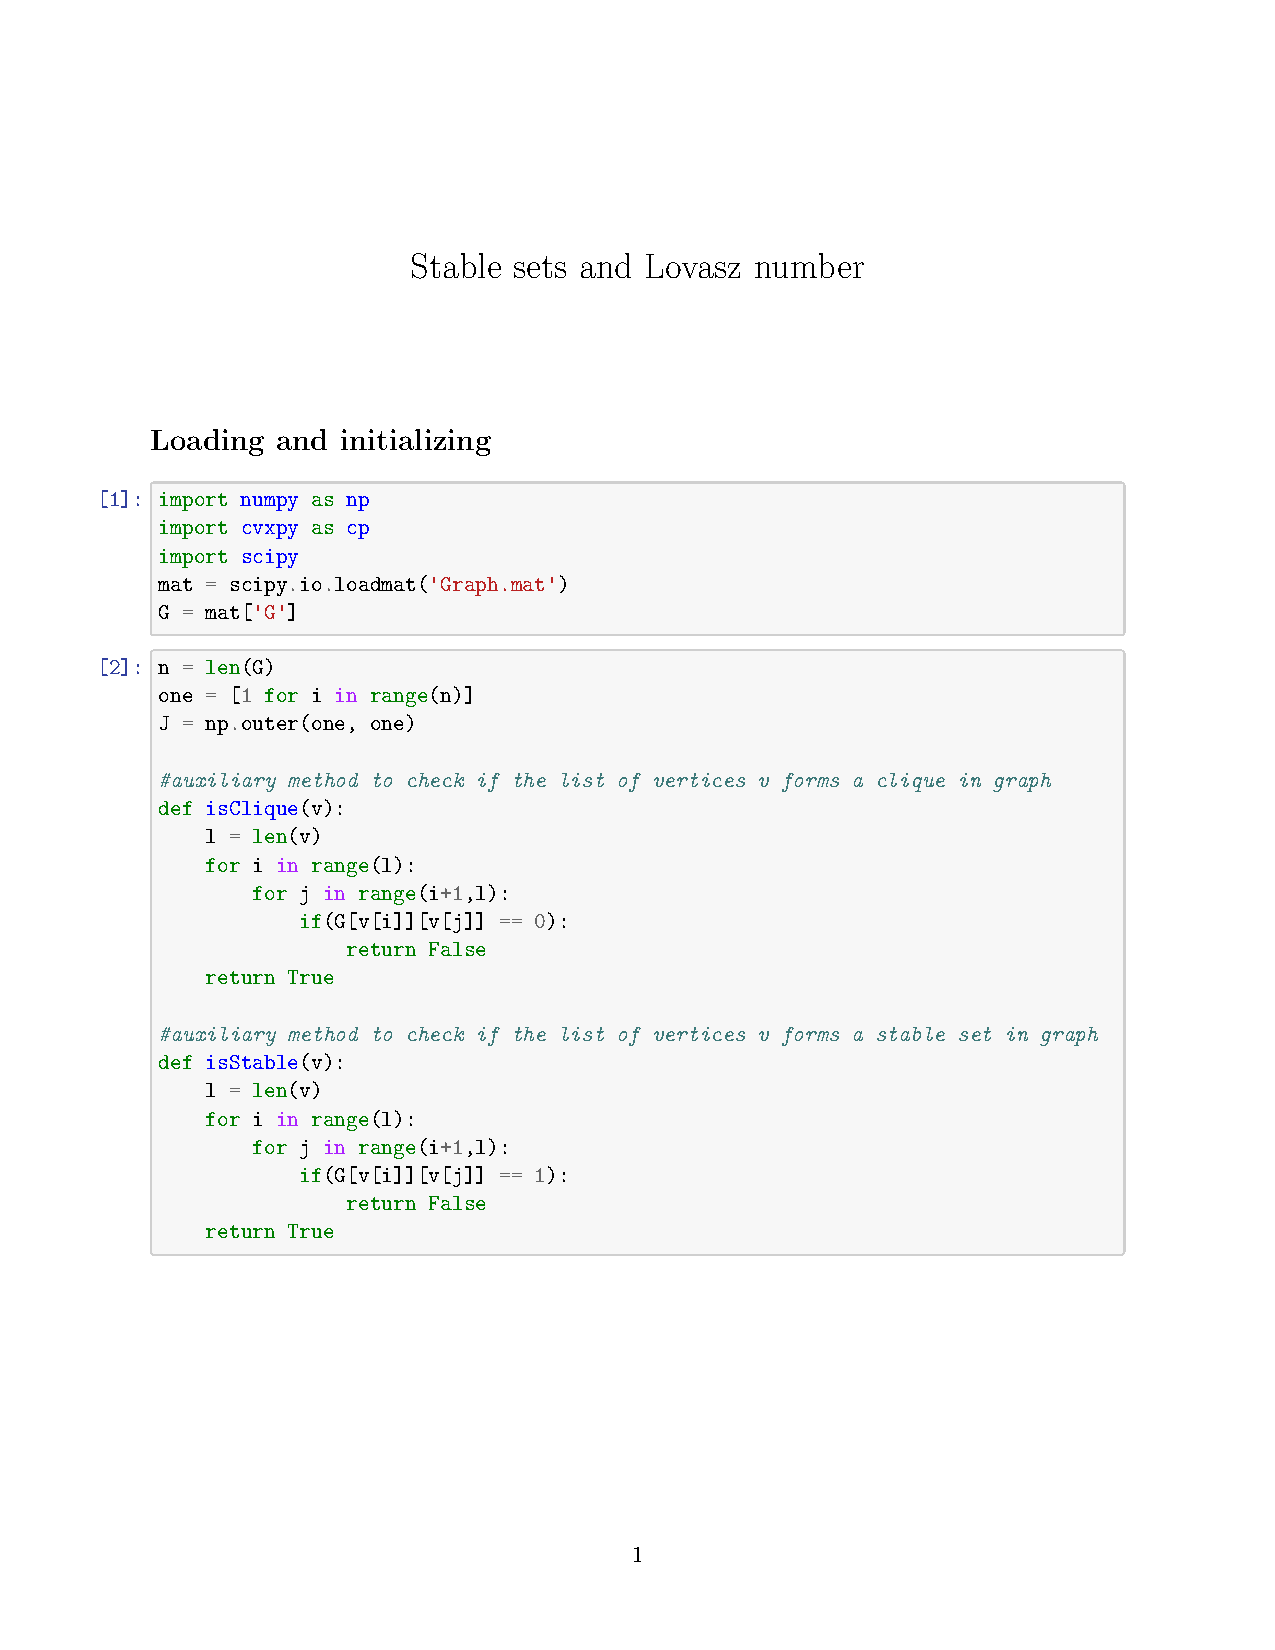
\includepdf[pages=-,pagecommand={\label{pdf:code}}]{graph/graph.pdf}}


\end{document}

